\documentclass{article}
\usepackage{settings}
\date{\today}
\begin{document}
\thispagestyle{empty}
\begin{center}
    \LARGE\textbf{МИНОБРНАУКИ РОССИИ\\
        САНКТ-ПЕТЕРБУРГСКИЙ ГОСУДАРСТВЕННЫЙ\\
        ЭЛЕКТРОТЕХНИЧЕСКИЙ УНИВЕРСИТЕТ\\
        "ЛЭТИ"\ ИМ. В.И.УЛЬЯНОВА(ЛЕНИНА)\\
        Кафедра МО ЭВМ}\\[4cm]
    \Large\textbf{ОТЧЁТ}\\[0.2cm]
    \Large\textbf{по учебной практике}\\[0.1cm]
    \Large\textbf{по дисциплине <<Генетические алгоритмы>>}\\[0.1cm]
    \Large\textbf{Тема: Алгоритм Рюкзака.}\\[2cm]
\end{center}
\Large{Студент гр. 1304 \qquad \qquad \quad \underline{\hspace{6cm}} \qquad \qquad Мусаев А.И.}\\[0.25cm]
\Large{Студент гр. 1304 \qquad \qquad \quad \underline{\hspace{6cm}} \qquad \qquad Поршнев Р.А.}\\[0.25cm]
\Large{Студентка гр. 1381 \qquad \quad \quad \underline{\hspace{6cm}} \qquad \qquad Демчук П.Д.}\\[0.25cm]
\Large{Преподаватель \qquad \qquad \qquad \underline{\hspace{6cm}} \qquad \qquad Жангиров Т.Р.}\\[1cm]
\begin{center}
    Санкт-Петербург\\
    2023
\end{center}
\newpage

\textbf{Задание}

Пусть имеется набор предметов, каждый из которых имеет два параметра — масса и ценность. Также имеется рюкзак определённой грузоподъёмности. Задача заключается в том, чтобы собрать рюкзак с максимальной (или близкой к максимальной) ценностью предметов внутри, соблюдая при этом ограничение рюкзака на суммарную массу.

\textbf{Выполнение работы}

\textbf{03.07 - 1 итерация}

\begin{enumerate}
\item GUI был спроектирован в Qt Designer. 

\begin{figure}[h!]
\centering
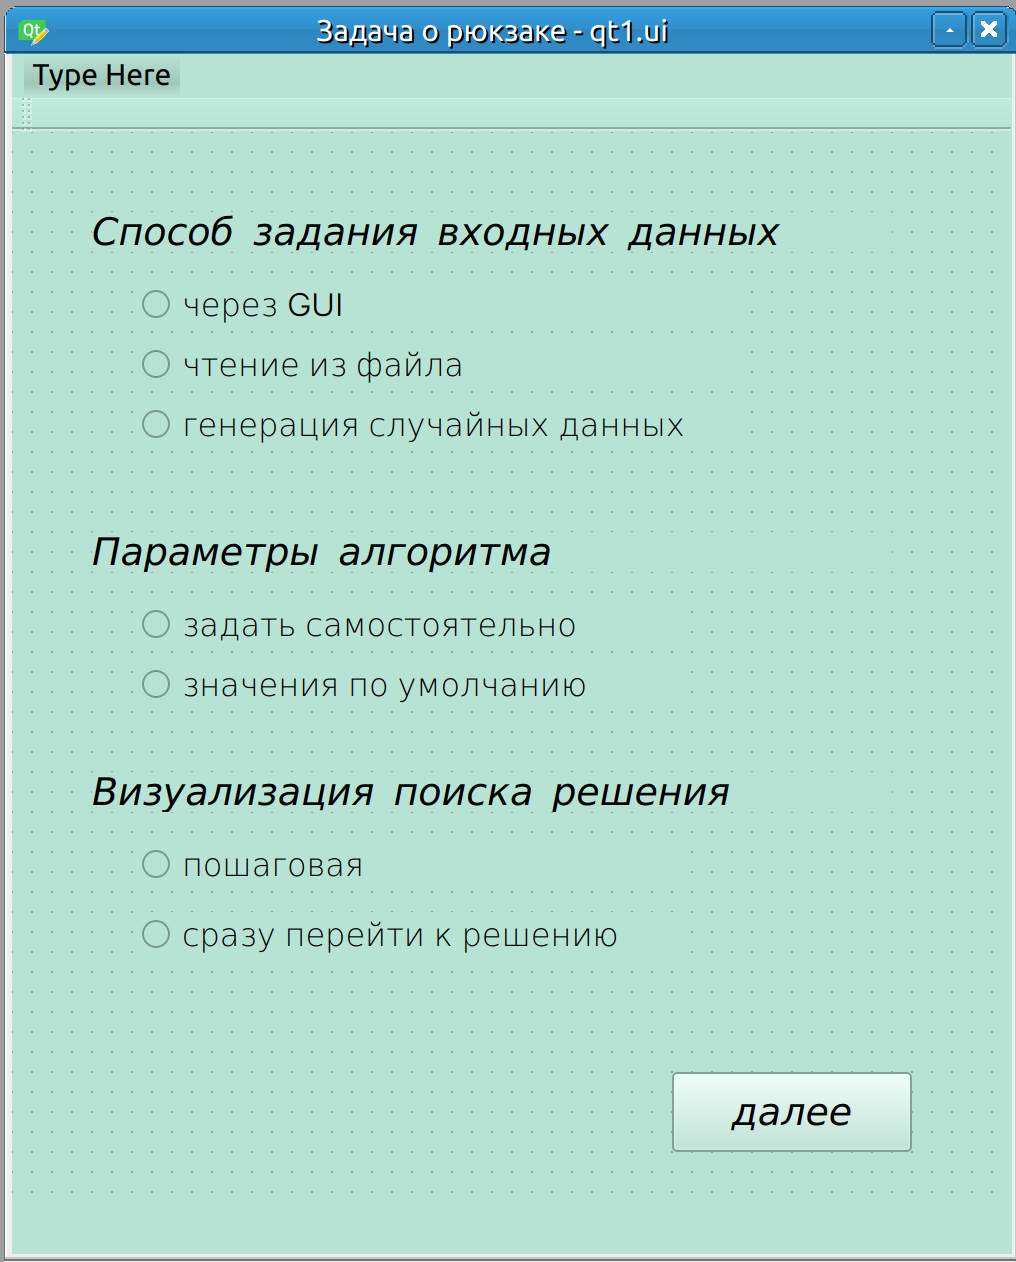
\includegraphics[width=0.5\linewidth]{images/qt1.png}
\caption{Начальная настройка работы с алгоритмом}
\label{fig:mpr}
\end{figure}

\begin{figure}[h!]
\begin{minipage}[h]{0.32\linewidth}
\center{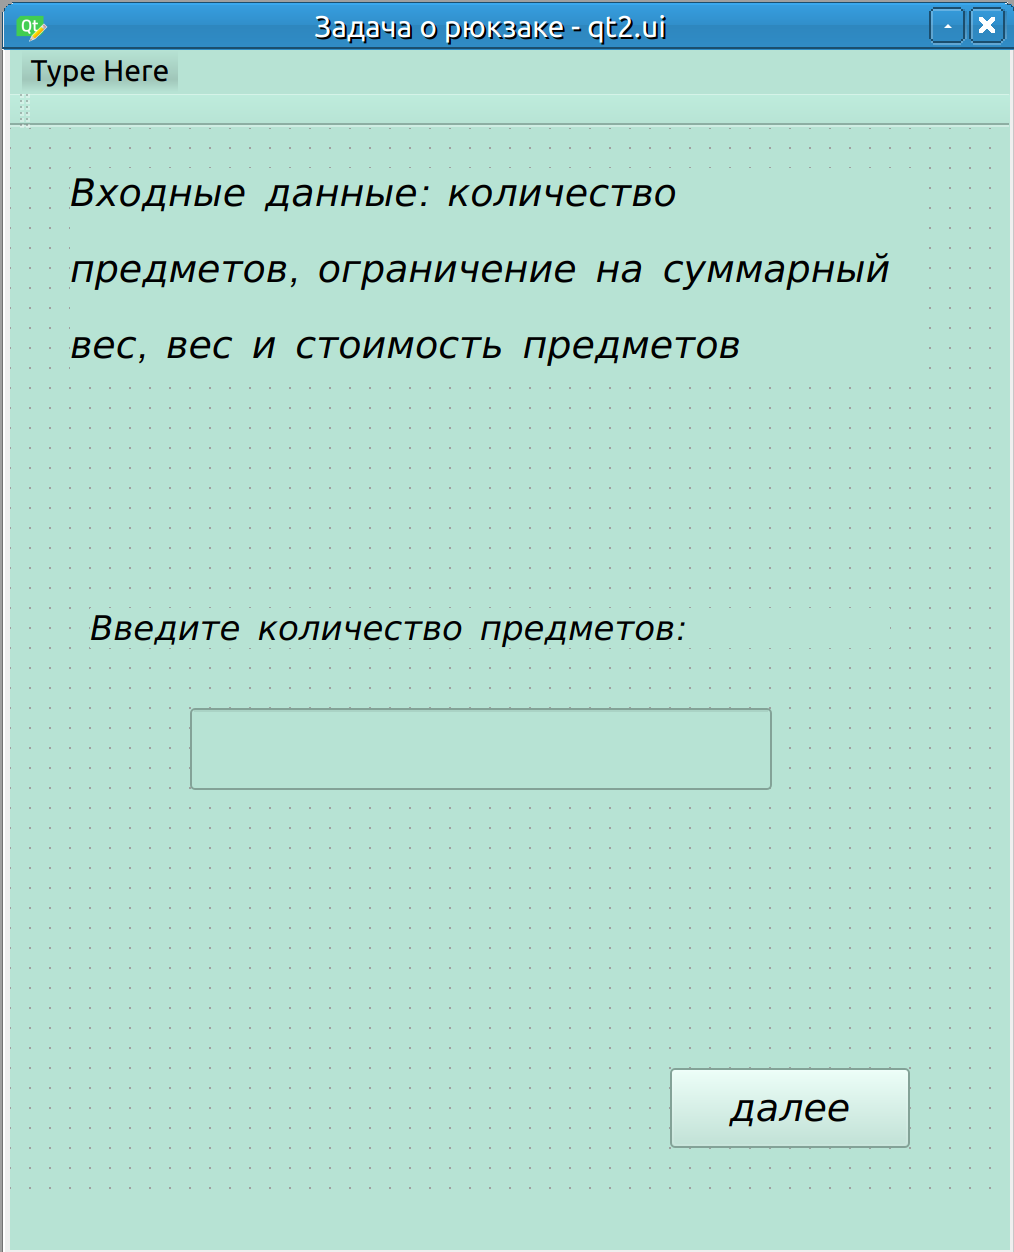
\includegraphics[width=1\linewidth]{images/qt2.png}}
\end{minipage}
\hfill
\begin{minipage}[h]{0.32\linewidth}
\center{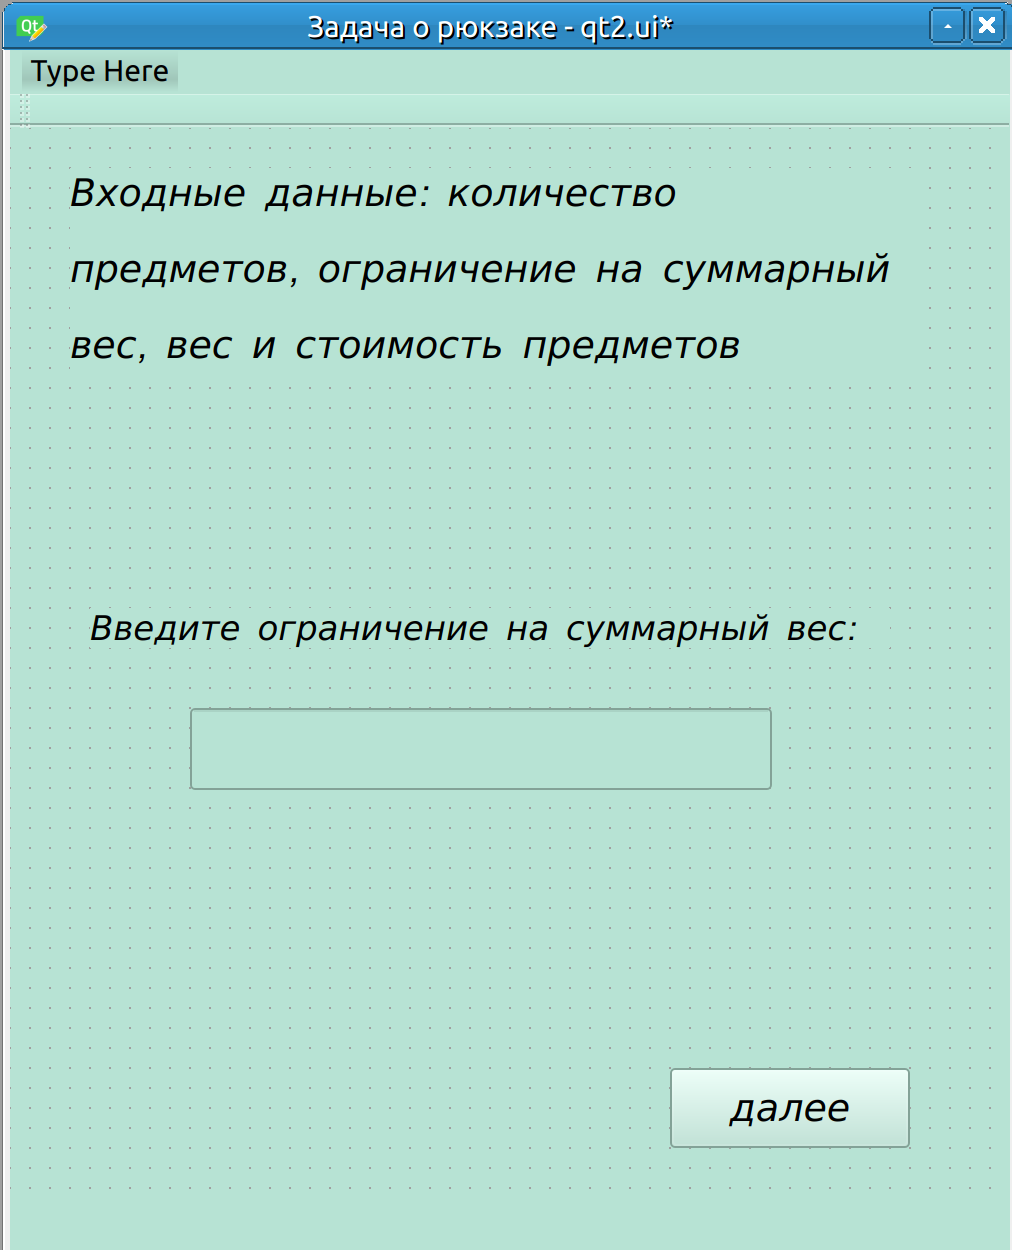
\includegraphics[width=1\linewidth]{images/qt2_2.png}}
\end{minipage}
\hfill
\begin{minipage}[h]{0.32\linewidth}
\center{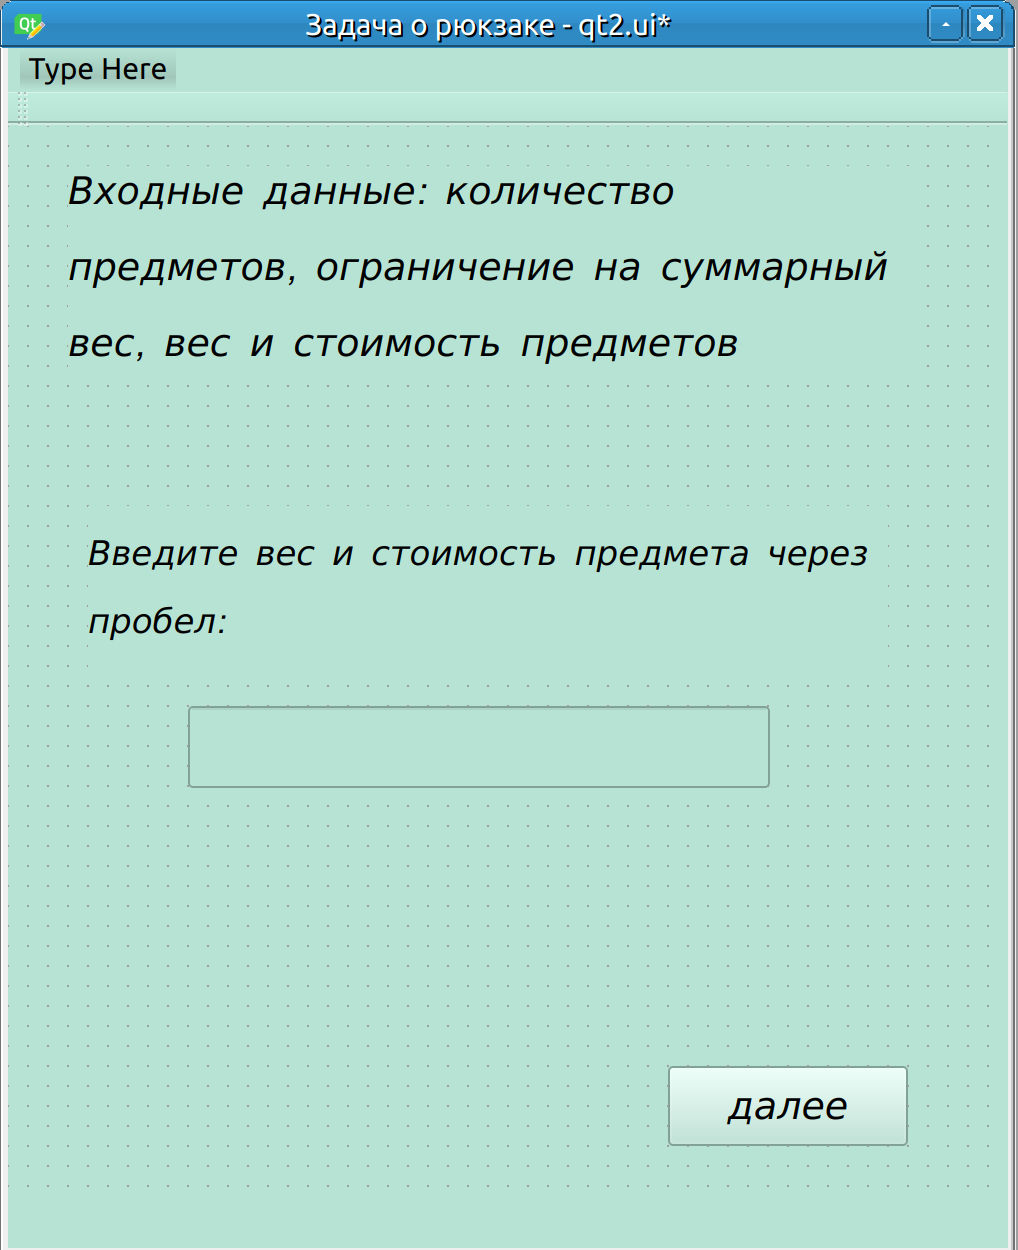
\includegraphics[width=1\linewidth]{images/qt2_3.png}}
\end{minipage}
\caption{Считывание входных данных}
\label{ris:image1}
\end{figure}

\begin{figure}[h!]
\begin{minipage}[h]{0.32\linewidth}
\center{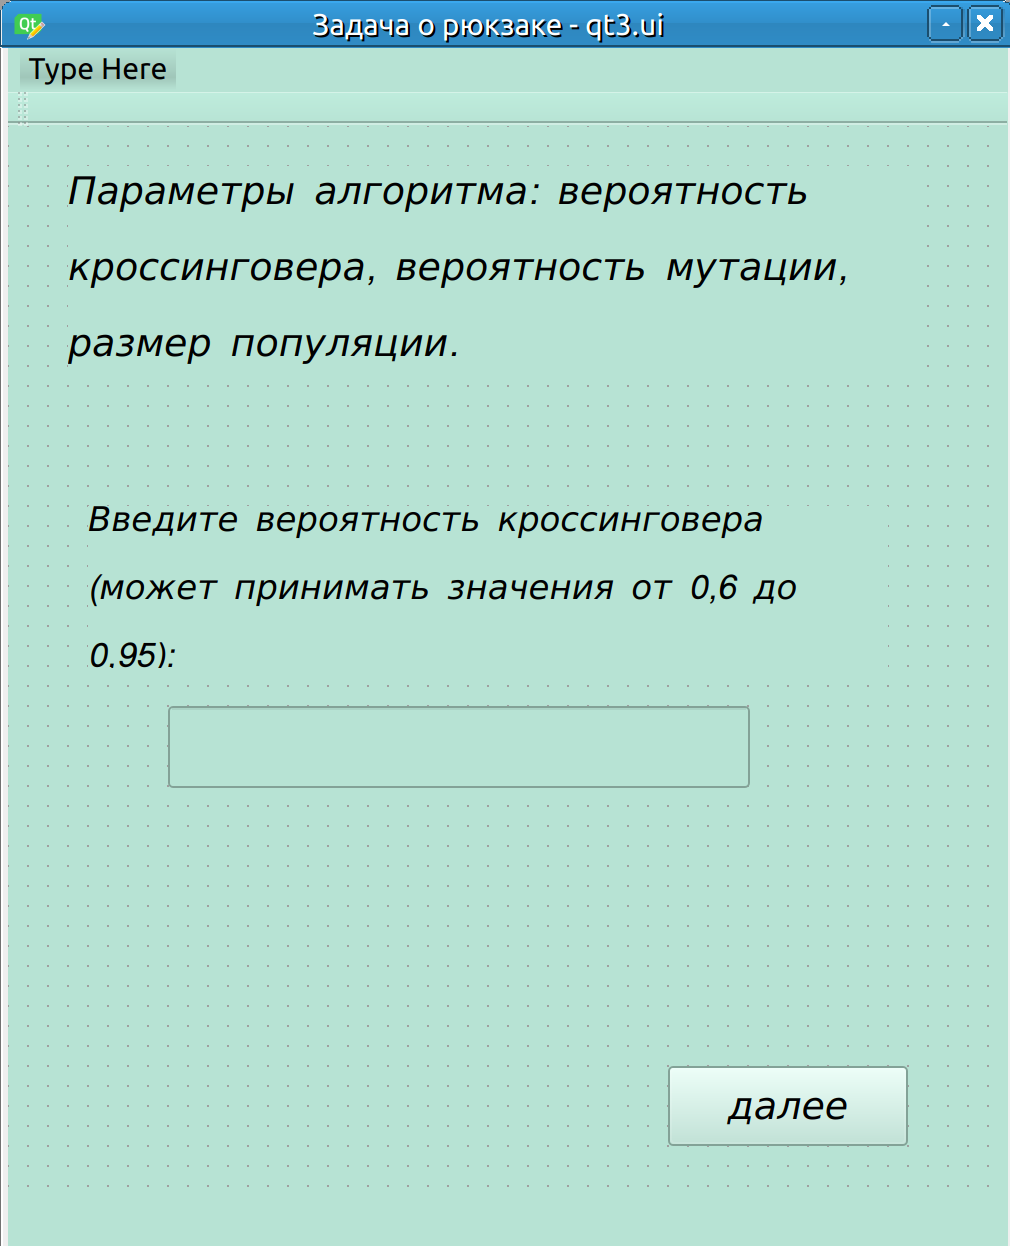
\includegraphics[width=1\linewidth]{images/qt3.png}}
\end{minipage}
\hfill
\begin{minipage}[h]{0.32\linewidth}
\center{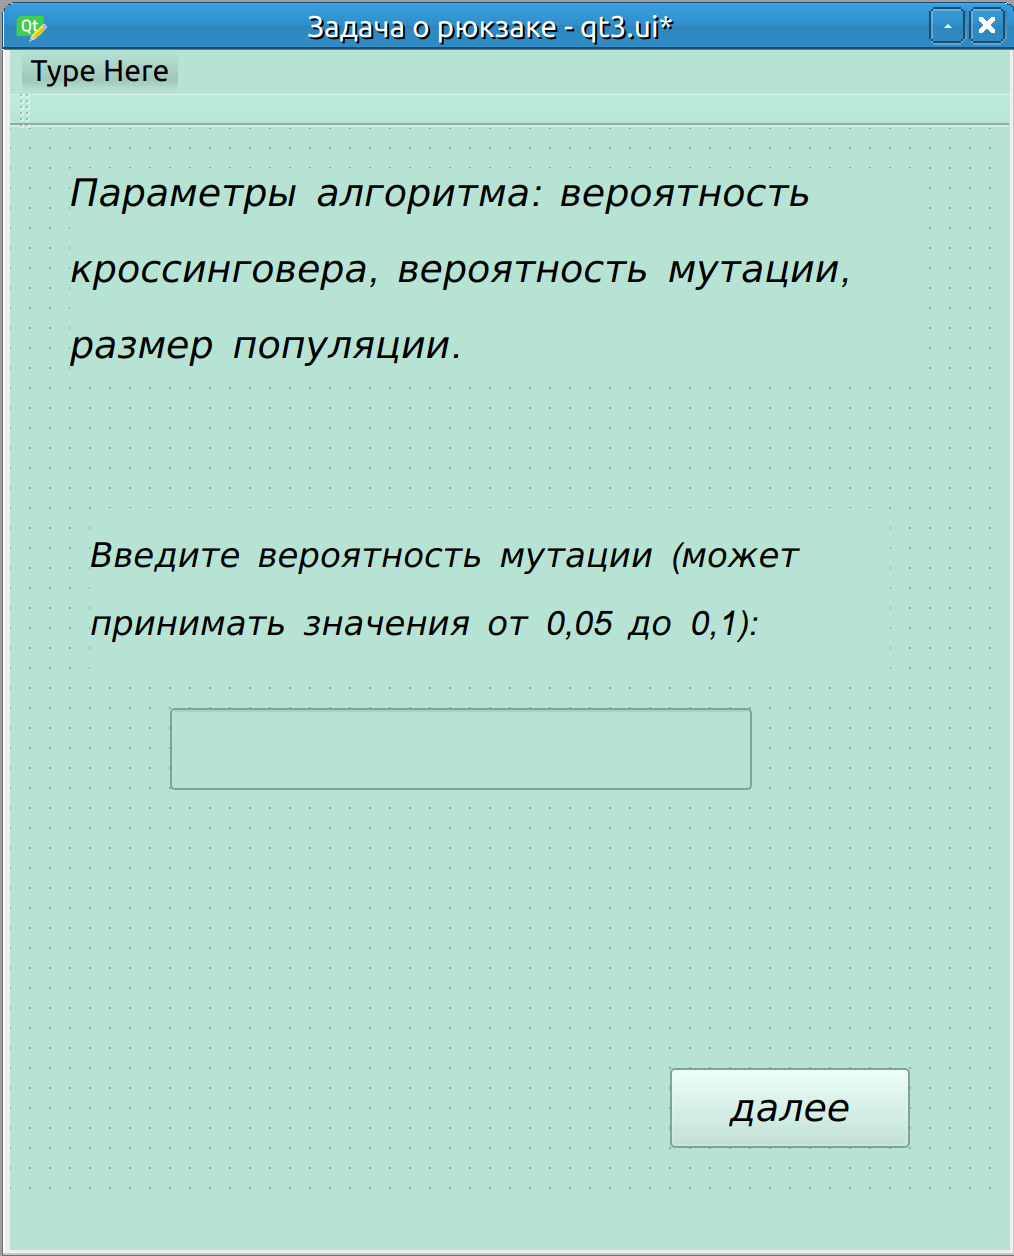
\includegraphics[width=1\linewidth]{images/qt3_2.png}}
\end{minipage}
\hfill
\begin{minipage}[h]{0.32\linewidth}
\center{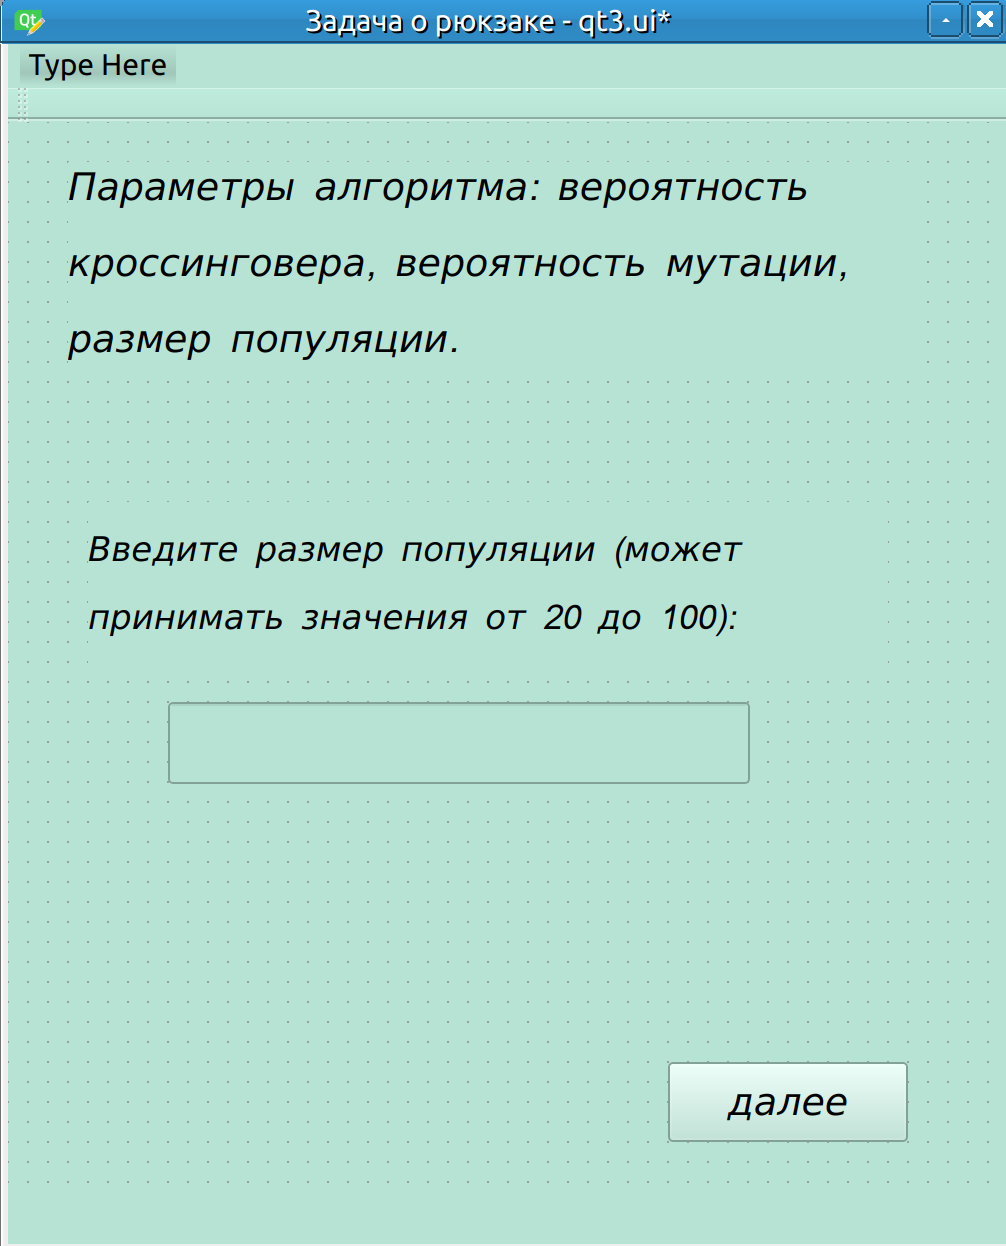
\includegraphics[width=1\linewidth]{images/qt3_3.png}}
\end{minipage}
\caption{Задание значений для работы алгоритма}
\label{ris:image1}
\end{figure}

\newpage

\item Модификации генетического алгоритма

Выбор родителей будет происходить турнирным отбором, так метод рулетки с большей вероятностью сведётся к жадному алгоритму, что невыгодно для решения задачи о рюкзаке.

Формирование пар родителей будет производиться сначала по принципу аутбридинга, а в конце работы алгоритма глобальные экстремумы будут уточняться по принципу инбридинга. 

Рекомбинация пар будет происходить при помощи однородного кроссинговера, так как данный способ гарантирует, что в строке-потомке будут чередоваться короткие строки особей-родителей. 

Мутация для каждой полученной особи будет происходить самоадаптирующимся способом при помощи критерия расстояния, то есть вероятность мутации каждого гена потомка будет равна: 

{
\Large
\begin{center}
$P_r(A,B) = M(A,B)M_m = (1 - dist(A,B))M_m$, где

$dist(A,B) = \frac{1}{n}\sum_{i=1}^n\frac{a_i-b_i}{max_i-min_i}^d$, $d=0,2$ и $M_m=0,9$
\end{center}
}

Для отбора популяции будет использоваться отбор вытеснением, так как данный способ даёт возможность собрать наиболее разнообразный рюкзак, то есть находить несколько глобальных экстремумов, а также данный способ является наиболее надёжным.

В дальнейшем будет добавлена возможность выбора методов, на основе которых выполняется генетический алгоритм.

\item Метрики генетического алгоритма

Пользователю будет предоставлена возможность задавать метрики самостоятельно либо по умолчанию. В случае задания вероятности кроссинговера самостоятельно её значения должно варьироваться в пределе от 0.6 до 0.95, для мутации - от 0.005 до 0.01 (в случае выбора самоадаптирующейся мутации данный функционал пользователю недоступен), а размер популяции - от 20 до 100 особей. По умолчанию будут использованы следующие метрики: вероятность мутации равна 0.01 (не применимо для самоадаптирующейся мутации), вероятность кроссинговера равна 0.8, размер популяции равен 30 особям.

\item Описание структур данных для хранения

Чтобы хранить поданные в генетический алгоритм данные будет использоваться массив кортежей, в котором каждому предмету будет соответствовать кортеж (цена, вес).

Для хранения отдельной хромосомы будет использован тип str, который будет хранить двоичное число (1 - предмет взять в данном наборе, 0 - отсутствует). Популяция же будет состоять из списка строк. Также будет использоваться список, каждый элемент которого будет хранить кортеж вида - (суммарная стоимость генотипа, суммарный вес генотипа). Оба вышеоуказанных массива будут храниться в структуре, которая характеризует популяцию. 

\item Стек технологий

Для реализации GUI будет использоваться библиотека PyQt, а для отрисовки графиков функции качества -- Matplotlib.

\item Распределение ролей в бригаде

Студент Мусаев Артур ответственный за проектировку и хранение данных, студентка Демчук Полина ответственная за разработку GUI, студент Поршнев Роман ответственный за разработку архитектуры.

\end{enumerate}

\newpage

\textbf{Заключение}

\textbf{01.07}

На данной итерации были частично распределены роли, выбраны модификации и метрики работы алгоритма. Разработана макет GUI. Кроме того, была создана архитектура проекта.

\end{document}

